\documentclass[]{article}
\usepackage{vub}

\title{Lazarus}
\subtitle{Group G21}
\author{Arno De Greef \& Andreas Declerck}

\faculty{Computerwetenschappen \& Ingenieurswetenschappen}

\promotors{Academic year 2021-2022}
\pretitle{Project Computersystemen}
\date{26 December 2021}
\usepackage{graphicx}

\usepackage{import}
\usepackage{pdfpages}
\usepackage{transparent}
\usepackage{xcolor}
\usepackage{hyperref}

\hypersetup{
    colorlinks=true,
    linkcolor=blue,
}

% enable utf-8 symbols
\usepackage[utf8]{inputenc}

\usepackage{parskip}

% Add fig command from Castel
\newcommand{\incfig}[2][1]{%
    \def\svgwidth{#1\columnwidth}
    \import{./figures/}{#2.pdf_tex}
}

\pdfsuppresswarningpagegroup=1

\begin{document}
\maketitle
\section{Introduction}

\begin{figure}[htpb]
    \centering
    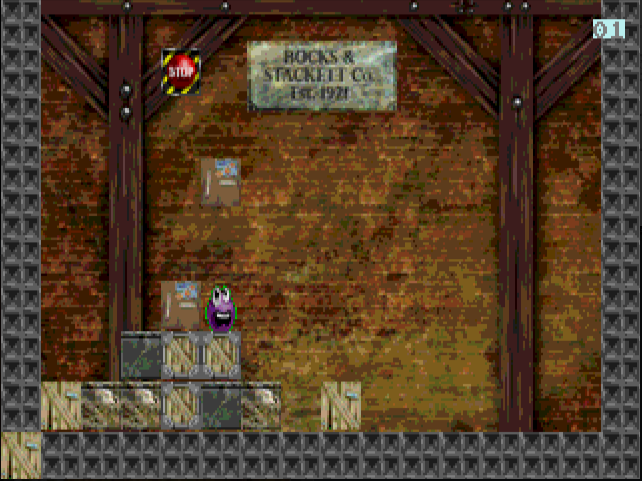
\includegraphics[width=0.6\linewidth]{figures/lazarus_spel.png}
    \caption{Lazarus game}
    \label{fig:lazarus_spel}
\end{figure}

You play as Lazarus, an innocent friendly blob, who was unfortunate 
enough to end up in a psychotic experiment where he needs to evade
falling boxes to reach the stop button in order to survive.

But be wary, boxes are not all made equal. Some are made from lesser 
materials and will break if heavier boxes crush them.

Being crushed by a box means game over.

The game was inspired by the game Lazarus from the book 'Games ontwerpen met
Game Maker' from Mark Overmars and Jacob Habgood\footnote{ISBN:
978-90-5940-284-3}.

\section{Manual}
The game starts with a welcome screen. By pressing one of the direction
arrow keys, you can start the game. You start at the first level.

Try and evade the falling boxes by moving left or right. Lazarus can 
only jump on crates that are 1 tile high and gets stuck if in between
2 high crate walls.

When you win, you go to a next screen from which you can continue to 
go to the next level by pressing the directional arrow keys. Losing 
resets all your progress back to level 1.

Press \emph{ESC} to stop the game at any time.

\section{Program features}
Crates have weight and can crush lighter crates. The player always knows
which type of crate will fall next by looking at the lower left corner. 
The X-coordinate of the falling crate is determined by where the player 
stands at the moment of creation, so the player can strategically 
choose where the next crate will land.

Every level the boxes will drop faster to increase the difficulty.
The player can fly when moving fast enough (handy when being stuck
in one part of the map) and when surviving long enough in the world,
the player receives matrix-like capabilities by slowing down the falling of the
crates when surviving long enough.

To prevent that every time you play feels the same, the destination button
moves to a different random location each time.

Progress is shown in the right upper corner with an indication of the
current level the player is in.

The game has custom sprites (the original sprites from the game Lazarus
from the book 'Games ontwerpen met Game Maker' from Mark Overmars and Jacob
Habgood) which are adapted to work with the reduced color space in the
\emph{Dosbox} environment. Transparency in the sprites is accomplished by
removing a green screen color.

The original sprites from the game Lazarus\footnote{\href{https://www.vanduurenmedia.nl/EAN/9789059402843/Leer_jezelf_MAKKELIJK_Games_ontwerpen_met_Game_Maker}{Downloadlink sprites}}:
\begin{figure}[htpb]
    \centering
    
\includegraphics[width=0.2\linewidth]{../sprites/Lazarus_stand.png}
    \caption{Lazarus stand}%
\end{figure}

\begin{figure}[htpb]
    \centering
    
\includegraphics[width=0.2\linewidth]{../sprites/Button.png}
    \caption{Stop button}%
\end{figure}

\begin{figure}[htpb]
    \centering
    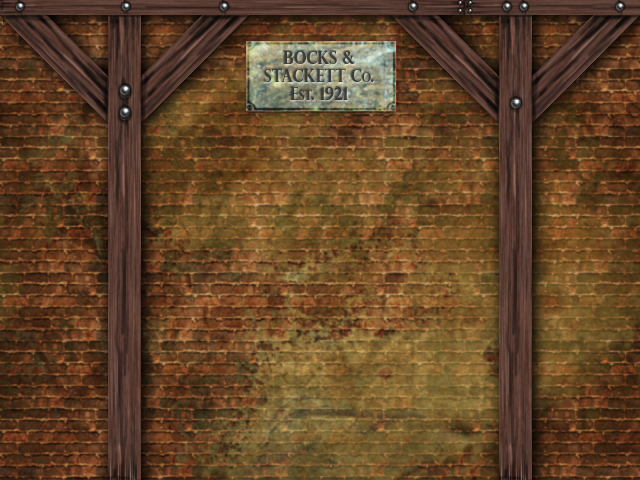
\includegraphics[width=0.4\linewidth]{../sprites/Background.png}
    \caption{Background of the game}%
\end{figure}

To make the game more engaging, the player looks scared when there is a crate
falling directly above him. This is a non functional feature, but makes the 
interaction with the game more appealing.

\section{Program design}

\subsection{High level overview}%
\label{sub:high_level_overview}

The game code exists of 6 different logically separated parts. Each of them
has its own file and its own role in the software architecture.

To visually separate the different procedures in the code, every procedure
starts with a prefix denoting the place where they were defined.

The game starts in \emph{main.asm} which controls the game loop and slows the
game down to wait for VBI which is better for VGA screens (sort of Vsync)

\subsection{Drawer}%
\label{sub:drawer}

All objects are are abstracted behind a drawable object that contains the
needed geometry with a pointer to the sprite data. Every time the sprite
updates, it needs to send its updated data to the drawer by make a call to be
redrawn.

In reality it is not actually directly written to the graphics buffer,
but to a back buffer that will be copied to the graphics buffer when all
drawing operations are done (double buffering). This prevents visual stuttering
caused by intermediate results of the drawn screen.

The drawer object is used in the entire program to abstract a game entity/tile.
This gives some sort of abstraction around an entity while also preventing the
overhead of having multiple abstractions for many other types (extra pointers).

\subsection{Physics}%
\label{sub:physics}

The game is tile based, but the falling of the crates can happen outside the
tiles, so there is no direct abstraction from the pixels to the tiles
representation. The conversion from tiles to pixels would also mean we would
need a multiplication which can be expensive if needed on every
iteration/entity.

To optimize the collision detection, the game separates the entities into 3
categories, implemented by 3 buffers:
\begin{itemize}
    \item Moving objects: Objects that can be moved and need to be recalculated
        every frame. This consists of the player.
    \item Static objects: Only collision is needed with moving objects but will
        never move on there own. These consist of the walls around the arena.
    \item Dynamic objects: Objects that mostly do not move but can be
        interacted with. They behave mostly as static objects but can interact
        (need collision detection) with moving objects. These are the crates
        who need to be able to be destroyed.
\end{itemize}

Gravity is implemented with a mass which is implemented more as a velocity than
an acceleration. This is to keep the game implementation simple while still
keeping a close enough resemblance to the impact of a real mass.

Collision is checked every frame. To make it efficient, only a few test points
are checked. One on top, one below, one left, one right and one in the middle.
The points are chosen in a way that going through crates is not possible, but
makes it possible to go back on a tile when moving fast enough. This creates
a more forgiving behavior for wrong input and makes the game feel more 
flexible.

\subsection{Crates}%
\label{sub:crates}

Crates are spawned when the crate timer runs out. Every new crate is spawned
at the top of the arena with the X-coordinate of the player. This to make
the spawning of the crates predictable, so the player can make plans to
position itself strategically. The next crate type will always be shown in the 
lower left corner. The type and its corresponding weight is encoded with the
position in memory of its sprite.

When one crate falls on top of another crate and the crate below is lighter
than the crate on top, the lower will break (removed from the game, aka crate
dynamics). The lower crate always looks above itself and checks the weight 
condition which relies on the sprite offset lead out in memory.

Sprites are dynamically loaded from disk and assigned to at startup initialized
memory.

\subsection{Player}%
\label{sub:player}

When the player updates and receives a key press event from the game (see
section \ref{sub:game}), it makes the necessary checks to see if it can move
left or right. If it can't, the player is raised one tile higher to see if it
can go left or right. If it can, it will make the move resulting in a jump of
1 tile high. Else the player's position is restored to the original one before,
effectively canceling the movement. Since the input events are way faster than
what feels normal for an update on every event, a timer was introduced that
slows down the input to only one input event for every few frames (the rest 
is discarded).

Every update, the player sends a request with its X-coordinate to spawn a new
falling crate. The spawning will only succeed depending on the crate timer 
(see section \ref{sub:crates}). If the spawning succeeds the X-coordinate is
stored by the player and every time the player has the same X-coordinate as 
the falling crate, its sprite changes to a scared version.

\begin{figure}[htpb]
    \centering
    
\includegraphics[width=0.2\linewidth]{../sprites/Lazarus_squished.png}
    \caption{Player scared}%
\end{figure}

The player checks every game iteration if he has won or lost. This is done by
checking for a collision with a crate just above him (loss) or by colliding in
the middle with the end button. If one of these 2 conditions is met, a signal
will be send to the game (see section \ref{sub:game}).

\subsection{Game}%
\label{sub:game}

The game manages the current state of the program and gets called every
iteration by main. It manages the menu and handles the raw button input.

When transitioning between states, an input delay is introduced, so the game 
would not immediately restart when going to a menu screen.

The game's update method starts by drawing the arena to the back buffer and 
initializes the physics registration of the walls (static). The sprites for the
walls are only defined for an area of 20x20 pixels, so the visual walls are consisting
of little blocks while the parts registered by the physics engine are 3 big
areas that function as an invisible collision box.

Next the game updates the entities by calling their corresponding update 
procedure, so they can draw themself to the back buffer.

The last step in the update procedure is drawing the text, since they are
drawn with interrupts directly to the screen and not to the back buffer.

These steps can vary depending on the current state of the game (playing, menu,
...)

When the game receives a message from the player when it has won or lost, the game
will clean all resources used during the playing of the game, set an input
delay timer and show the current status on the screen.

The cleaning is important, otherwise the game comes into an infinite loop where
it tries to restart itself but gets immediately a loss/win message from the
player.

Whenever the game checks for new input, it looks if the current key is not 
\emph{ESC} and if true exits the game by returning from the update procedure
with $eax \neq 0$ (handled by main which ends the program).

To prevent boxes from colliding with the final button, the button is not added
to one of the physics buffers, but checked manually in the player (using a
procedure of the physics).

\subsection{Dynamic data layout}%
\label{sub:dynamic_data_layout}

In the game, crates can be destroyed and created dynamically. This is why we 
need a dynamic buffer-like structure to be able to (de)allocate the crates and
their corresponding physics representation.

This is accomplished by preallocating an array of uninitialized memory and 
another array consisting of bitflags that indicate which location in the 
uninitialized memory is currently in use or not.

To help work with these buffers, some procedures where written in
\emph{utils.asm}. These consist of finding a free spot, in the buffer to place
an entity, a procedure to set the state of a spot and some procedures to add
and remove an entity from the buffer.

\section{Encountered problems}

The original sprites are gifs encoded with a reduced color space and were
animated. This posed a problem since this is not easy to draw to a screen with 
the given available system calls. So we had to first increase the color space 
to full \emph{RGB} and put all the images we wanted to use in one big atlas to
be able to reduce the color palette again to something that is compatible with
\emph{Dosbox}. Getting all the bits correct was challenging.

The initial set of points to be checked during the collision detection allowed
the player in some situations to get stuck inside a crate. Finding and 
optimizing the points eventually improved the glitchy behavior to something 
that is more pleasant to play with.

Some unfamiliarity with assembly made us make some stupid mistakes like adding
for example \emph{eax} to the USES directive while also trying to return a
result from the corresponding procedure or ending a procedure without writing
the \emph{ret}-instruction.

\section{Conclusion}

The basic functionality is where it needs to be with most of the original
features of the game implemented. Features that where not implemented where
things like a more advanced leveling system with more variety in level design
and background music with corresponding animations.

After all we are happy with the end result and the complexity of the current 
implementation.

\end{document}
